 \thispagestyle{gocconone}
\pagestyle{gocco}
\everymath{\color{gocco}}
\graphicspath{{../gocco/pic/}}
\blfootnote{$^1${\color[named]{gocco}Đại kiện tướng quốc tế.}}
\begingroup
\AddToShipoutPicture*{\put(0,616){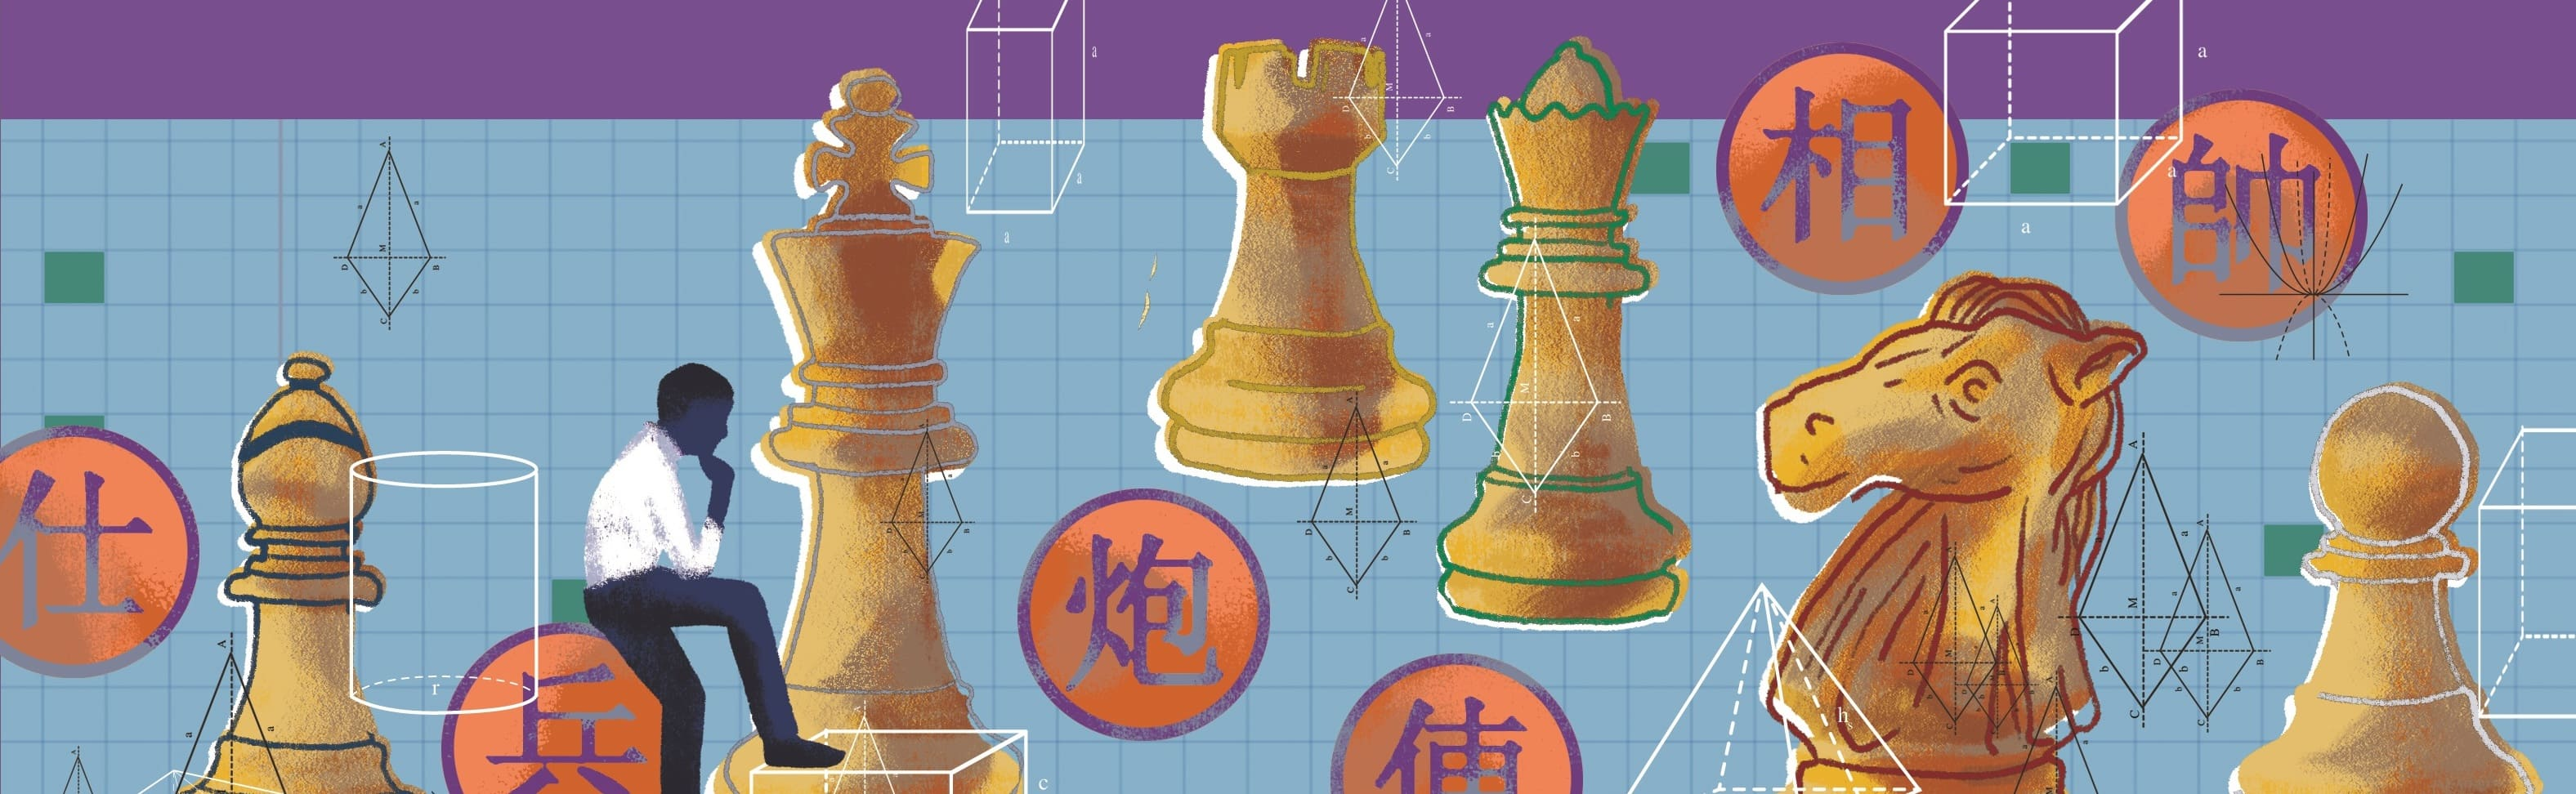
\includegraphics[width=19.3cm]{../bannergocco}}}
\AddToShipoutPicture*{\put(104,555){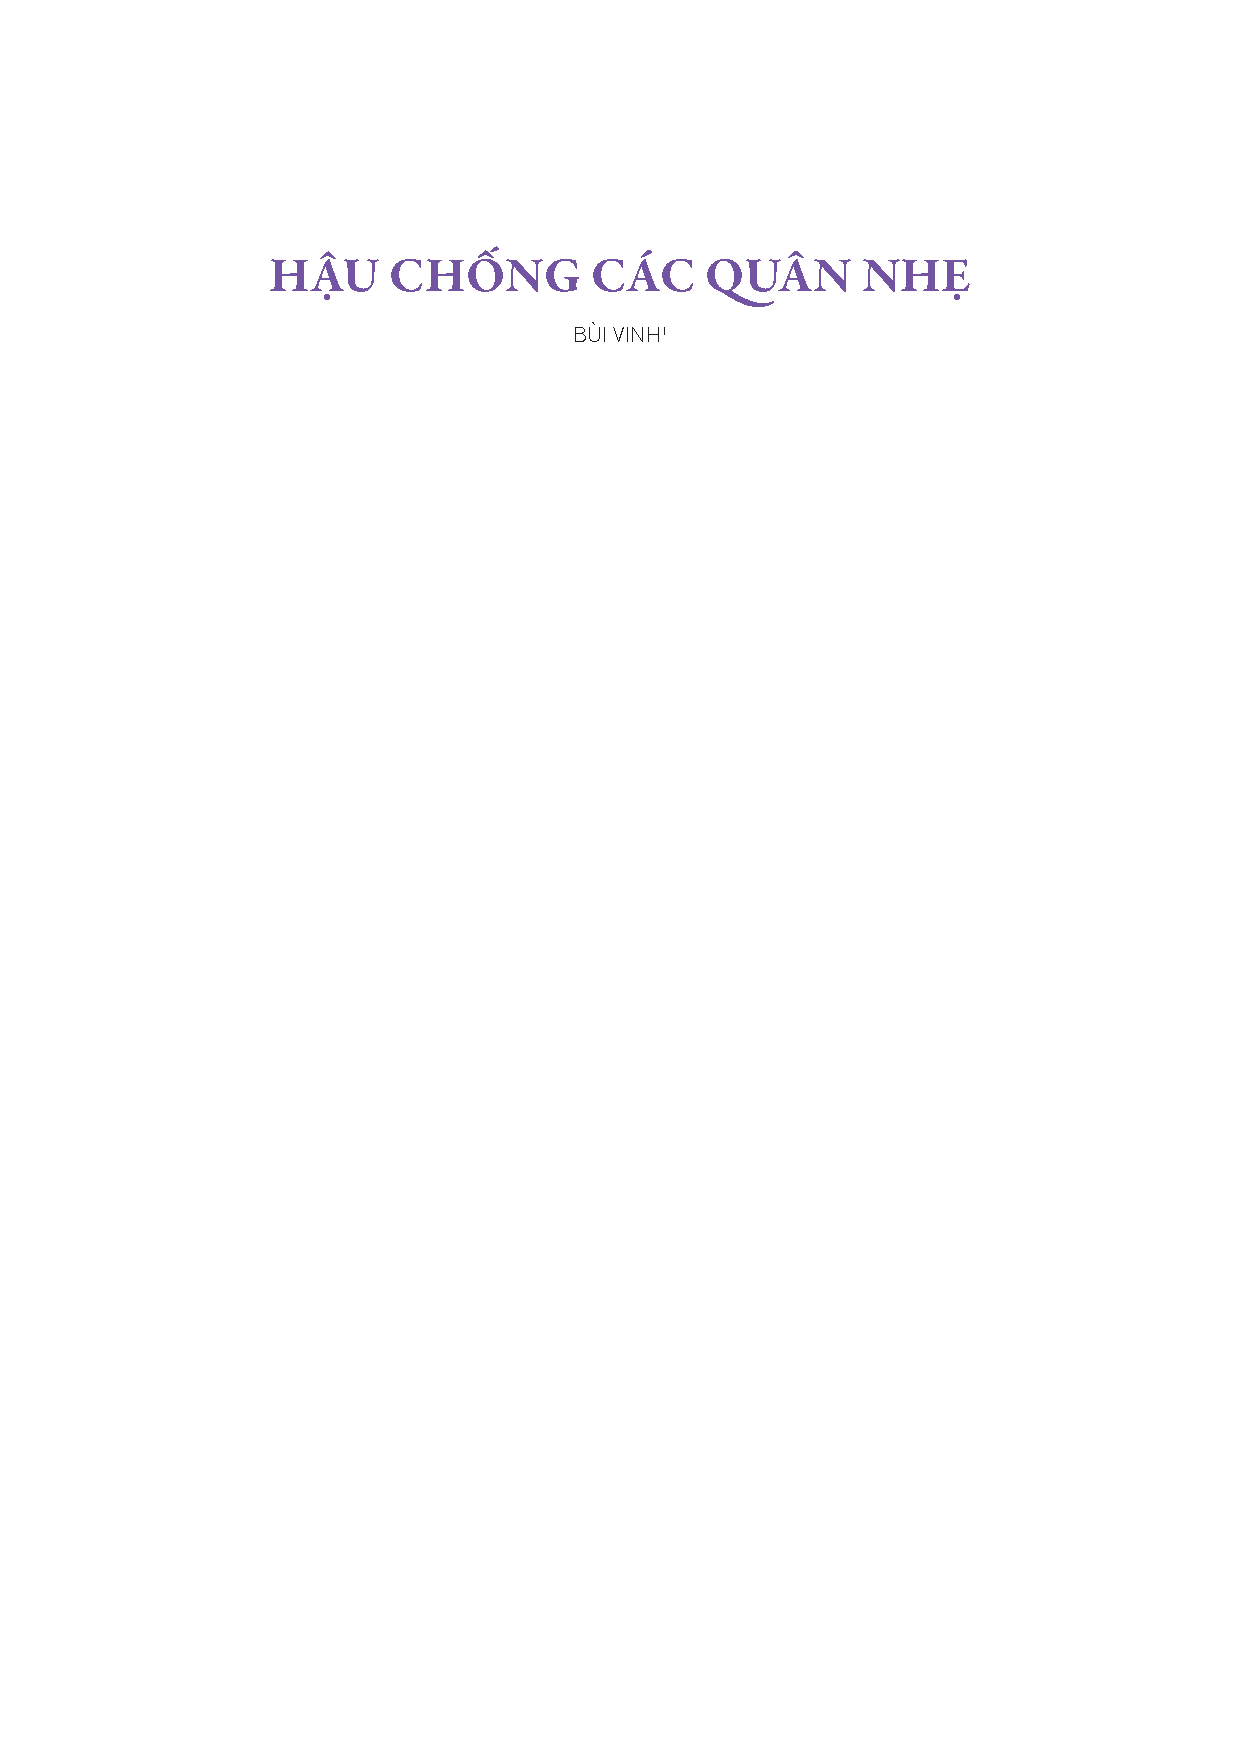
\includegraphics[scale=1]{../tieude.pdf}}} 
\centering
\endgroup

\vspace*{150pt}

\begin{multicols}{2}
	Lý thuyết cờ tàn cơ bản đều cho rằng Hậu sẽ dễ dành chiến thắng trong khi chống lại các quân nhẹ.
	\vskip 0.1cm
	Trong bài học hôm nay, chúng ta sẽ xem xét một vài tình huống có tính chất tiêu chuẩn như sau:
	\vskip 0.1cm
	$1.$ \textit{Trường hợp Hậu chống lại hai tượng.}
	\vskip 0.1cm 
	Hai tượng trong cờ tàn rất mạnh vì khả năng che chắn và làm hàng rào ngăn chặn vua đối phương. 
	\vskip 0.1cm
	Tuy nhiên khi không còn tốt, Tượng sẽ rất khó tránh khỏi nước chiếu bắt đôi của Hậu.
	\vskip 0.1cm
	Lý thuyết chỉ ra rằng có hơn $90\%$ các thế cờ bên có Hậu sẽ giành chiến thắng.
	Chúng tôi sẽ trình bày một vài tình huống cho chủ đề này.
	\vskip 0.1cm
	\textbf{\color{gocco}NN--NN}
	\begin{center}
		\newgame
		\fenboard{8/1k2K3/bb2Q3/8/8/8/8/8 b Q - 0 1}
		\scalebox{0.95}\showboard
		\vskip 0.1cm
		\textit{\small\color{gocco}Hình $1$.}
	\end{center}
	Chiến lược chơi cơ bản của Trắng là từ từ tiếp cận vua vào gần vua đối phương và buộc đối phương phải di chuyển một trong hai con tượng ra khỏi vị trí vua có thể bảo vệ được.
	\vskip 0.1cm
	$\pmb{1.}$\textbf{\color{gocco}Vd}$\pmb{7}$
	\vskip 0.1cm
	$\pmb{1}$\textbf{\color{gocco}...Tb$\pmb{5+}$ $\pmb{2.}$Vd$\pmb{6}$ Ta$\pmb{7}$} Mọi phương án khác của đen đều dẫn đến Trắng chiếu bắt tượng như:
	\vskip 0.1cm
	$2$...Tc$7+$ $3$.Vc$5$ Ta$4$ $4$.He$4+$ Đen bị mất Tượng; $2$...Vb$8$ $3$.Hb$3$; $2$...Ta$4$ $3$.He$4+$; $2$...Va$7$ $3$.Hc$8$ Đen bị hết nước đi $3$...Ta$6$ $4$.Hd$7+$ Tb$7$ $5$.Ha$4+$ Vb$8$ (\textit{$5$...Ta$6$ $6$.Vc$6$ Tg$1$ $7$.Hb$4$ Tf$2$ $8$.He$7+$ Va$8$ $9$.Hf$8+$}) $6$.Vd$7$ Ta$8$ $7$.Ha$6$ Tc$7$ (\textit{$7$...Te$3$ $8$.Hb$5+$ Va$7$ $9$.Ha$4+$ Vb$8$ $10$.Hb$3+$}) $8$.Hc$8+$
	\vskip 0.1cm
	$\pmb{3}$\textbf{\color{gocco}.He$\pmb{7+}$ Vb}$\pmb{6}$  Nếu $3$...Va$6$ $4$.Hc$7!$ 
	\begin{center}
		\newgame
		\fenboard{8/b1Q5/k2K4/1b6/8/8/8/8 b Q - 0 1}
		\scalebox{0.95}\showboard
		\vskip 0.1cm
		\textit{\small\color{gocco}Hình $2$.}
	\end{center}
	$4$...Tb$6$ $5$.Hc$8+$ Va$7$ $6$.Hg$8$ Vb$7$ $7$.Hd$5+$ Va$6$ $8$.Ha$8+$ Ta$7$ $9$.Vc$7!$ 
	\begin{center}
		\newgame
		\fenboard{Q7/b1K5/k7/1b6/8/8/8/8 b Q - 0 1}
		\scalebox{0.95}\showboard
		\vskip 0.1cm
		\textit{\small\color{gocco}Hình $3$.}
	\end{center}
	Đen sẽ buộc phải di chuyển Tượng khỏi ô b$5$ và Trắng sẽ chiếu bắt mất Tượng sau vài nước
	\vskip 0.1cm
	$\pmb{4}$\textbf{\color{gocco}.Hc$\pmb{7+}$ Va$\pmb{6}$ $\pmb{5}$.Vd}$\pmb{5}$ Trắng tạo cho Vua đen hết nước đi, từ đó bắt buộc một trong hai tượng của đen phải di chuyển ra xa vua của mình.
	\vskip 0.1cm
	$\pmb{5}$\textbf{\color{gocco}...Tb$\pmb{6}$ $\pmb{6}$.Hc$\pmb{8+}$ Va}$\pmb{7}$ Nếu $6$...Va$5$ $7$.Ha$8+$ Ta$6$ ($7$...Vb$4$ $8$.Hf8$+$  Ka$4$ $9$.He$7!$ Ta$5$ $10$.Ha$7!$ Vb$4$ $11$.Hc$5+$ Va$4$ $12$.Hc$2+$ Va$3$ $13$.Hc$1+$ Vb$3$ $14$.Hb$1+$ Va$4$ $15$.Ha$2+$ Vb$4$ $16$.Hb$2+$ Va$4$ $17$.Vc$5$
	 \vskip 0.1cm
	Trắng thắng 
	\begin{center}
		\newgame
		\fenboard{8/8/8/bbK5/k7/8/1Q6/8 b Q - 0 1}
		\scalebox{0.95}\showboard
		\vskip 0.1cm
		\textit{\small\color{gocco}Hình $4$.}
	\end{center}
	$\pmb{7}$\textbf{\color{gocco}.Vd$\pmb{6}$! Ta$\pmb{6}$ $\pmb{8}$.Hc$\pmb{2}$ Tb$\pmb{7}$ $\pmb{9}$.Ha$\pmb{2+}$ Vb$\pmb{8}$ $\pmb{10}$.Vd}$\pmb{7!}$ 
	\begin{center}
		\newgame
		\fenboard{1k6/1b1K4/1b6/8/8/8/Q7/8 b Q - 0 1}
		\scalebox{0.95}\showboard
		\vskip 0.1cm
		\textit{\small\color{gocco}Hình $5$.}
	\end{center}
	Các phương án tiếp theo Đen sẽ thua vì không thể tránh khỏi mất tượng.
	\vskip 0.1cm
	$\pmb{10}$\textbf{\color{gocco}...Td$\pmb{4}$ $pmb{11}$.Hb$\pmb{3}$! Te$\pmb{5}$} Nếu $11$...Va$8$ $12$.Ha$4+$ Ta$7$ $13$.Vc$7$; $11$...Tf$2$ $12$.Hg$8+$ Va$7$ $13$.Ha$2+$; $11$...Tg$1$ $12$.Hg$8+$; $11$...Tf$6$ $12$.Hg$3+$ Va$7$ $13$.Vc$7$ trắng thắng
	\vskip 0.1cm
	$\pmb{12}$.Hb$\pmb{4!}$ Tg$\pmb{7}$ Các phương án khác cũng không thể tốt tránh khỏi nước chiếu bắt tượng $12$...Th$2$ $13$.Hf$8+$ Va$7$ $14$.Hf$2+$; $12$...Ta$1$ $13$.Hf$8+$ Va$7$ $14$.Ha$3+$
	\vskip 0.1cm
	$\pmb{13}$\textbf{\color{gocco}.He$\pmb{7!}$ Ta}$\pmb{1}$  Nếu $13$...Tc$3$ $14$.Hf$8+$ Va$7$ $15$.Ha$3+$; $13$...Tb$2$ $14$.Hf$8+$ Va$7$ $15$.Hf$2+$
	\vskip 0.1cm
	$\pmb{14}$\textbf{\color{gocco}.Hf$\pmb{8+}$ Va$\pmb{7}$ $\pmb{15}$.Ha}$\pmb{3+}$ Trắng thắng
	\vskip 0.1cm
	\textbf{\color{gocco}G. Lolli} $\pmb{1763}$
	\begin{center}
		\newgame
		\fenboard{8/1k6/1bb5/8/1K5Q/8/8/8 b Q - 0 1}
		\scalebox{0.95}\showboard
		\vskip 0.1cm
		\textit{\small\color{gocco}Hình $6$.}
	\end{center}
	Trong một vài tính huống đặc biệt, bên có hai tượng có thể gỡ hòa nhờ xây dựng các ``bong ke" hay ``lô cốt" không cho vua bên có Hâu tiếp cận hai tượng. Tuy nhiên bên có hai tượng phải phòng thủ rất chính xác.
	\vskip 0.1cm
	$\pmb{1}$\textbf{\color{gocco}.He$\pmb{7+}$ Vb}$\pmb{8!}$ Biện pháp phòng thủ tốt nhất cho đen.
	\vskip 0.1cm
	Nếu $1$...Tc$7$ $2$.Vc$5$! Th$1$ $3$.Hh$7$ Tg$2$ $4$.Hg$6$ Tf$3$ $5$.Hb$1+$ Vc$8$ $6$.Hf$5+$ Đen mất tượng
	\vskip 0.1cm
	$\pmb{2.}$Hd$\pmb{6+}$ Vb$\pmb{7}$ $\pmb{3}$.Vc$\pmb{4}$ Ta$\pmb{7}$ $\pmb{4}$.He$\pmb{7+}$ Vb$\pmb{6}$ $\pmb{5}$.Hd$\pmb{8+}$ Vb$\pmb{7}$ $\pmb{6}$.Vb$\pmb{4}$ Tb$\pmb{6}$ $\pmb{7}$.Hd$\pmb{6}$ Ta$\pmb{7!}$
	\vskip 0.1cm 
	Đen kiên quyết không rời tượng ra khỏi vua. Hai tượng đen tạo ra $1$ hàng rào ngăn vua trắng tiếp cận vua đen 
	\begin{center}
		\newgame
		\fenboard{8/bk6/2bQ4/8/1K6/8/8/8 b Q - 0 1}
		\scalebox{0.95}\showboard
		\vskip 0.1cm
		\textit{\small\color{gocco}Hình $7$.}
	\end{center}
	$\pmb{8}$\textbf{\color{gocco}.He$\pmb{7+}$ Vb$\pmb{6}$ $\pmb{9}$.Hd$\pmb{8+}$ Vb$\pmb{7}$ $\pmb{10}$.Va$\pmb{5}$ Tc$\pmb{5}$! $\pmb{11}$.Hf$\pmb{6}$ Tb$\pmb{6+}$ $\pmb{12}$.Vb$\pmb{4}$ Vc$\pmb{7}$
	\vskip 0.1cm 
	$\pmb{13}$.Vc$\pmb{4}$ Vb$\pmb{7}$ $\pmb{14}$.Hd$\pmb{6}$ Ta$\pmb{7}$ $\pmb{15}$.He$\pmb{7+}$ Vb$\pmb{6}$ $\pmb{16}$.Hd$\pmb{8+}$ Vb$\pmb{7}$ $\pmb{17}$.Vc$\pmb{3}$ Tb}$\pmb{6=}$ 
	\vskip 0.1cm
	Đen chơi chiến thuật chờ đợi.Trắng khổng thể có cách nào đưa vua tiếp cận hai tượng cũng như buộc bên đen phải di chuyển tượng khỏi vua. 
	\begin{center}
		\newgame
		\fenboard{3Q4/1k6/1bb5/8/8/2K5/8/8 b Q - 0 1}
		\scalebox{0.95}\showboard
		\vskip 0.1cm
		\textit{\small\color{gocco}Hình $8$.}
	\end{center}
	\textbf{\color{gocco}Bài tập về nhà}
	\vskip 0.1cm
	Trắng đi trước và thắng. NN
	\begin{center}
		\newgame
		\fenboard{8/5Q2/8/8/8/4K1bb/6k1/8 b Q - 0 1}
		\scalebox{0.95}\showboard
		\vskip 0.1cm
		\textit{\small\color{gocco}Hình $9$.}
	\end{center}
	Bài giải:
	\vskip 0.1cm
	$\pmb{1}$\textbf{\color{gocco}.Ha$\pmb{2+}$ Vg}$\pmb{1}$ Nếu $1$...Vh$1$ $2$.Vf$3$ Th$4$ $3$.Hd$2+–$
	\vskip 0.1cm
	$\pmb{2}$\textbf{\color{gocco}.Vf$\pmb{3}$ Th$\pmb{4}$ $\pmb{3}$.He$\pmb{2}$!} Phương án khác cũng dẫn đến Trắng thắng như sau $3$.Hd$2$! Vh$1$ $4$.Hb$2$! Vg$1$ $5$.Hd$4+$ Vh$1$ $6$.Hxh$4$
	\vskip 0.1cm
	$\pmb{3}$\textbf{\color{gocco}...Vh$\pmb{1}$ $\pmb{4}$.Hb$\pmb{2}$! Vg$\pmb{1}$ $\pmb{5}$.Hd}$\pmb{4+}$ Trắng thắng
\end{multicols}




